%% This is file `elsarticle-template-1a-num.tex',
%%
%% Copyright 2009 Elsevier Ltd
%%
%% This file is part of the 'Elsarticle Bundle'.
%% ---------------------------------------------
%%
%% It may be distributed under the conditions of the LaTeX Project Public
%% License, either version 1.2 of this license or (at your option) any
%% later version.  The latest version of this license is in
%%    http://www.latex-project.org/lppl.txt
%% and version 1.2 or later is part of all distributions of LaTeX
%% version 1999/12/01 or later.
%%
%% The list of all files belonging to the 'Elsarticle Bundle' is
%% given in the file `manifest.txt'.
%%
%% Template article for Elsevier's document class `elsarticle'
%% with numbered style bibliographic references
%%
%% $Id: elsarticle-template-1a-num.tex 151 2009-10-08 05:18:25Z rishi $
%% $URL: http://lenova.river-valley.com/svn/elsbst/trunk/elsarticle-template-1a-num.tex $
%%
\documentclass[preprint,12pt]{elsarticle}

%% Use the option review to obtain double line spacing
%% \documentclass[preprint,review,12pt]{elsarticle}

%% Use the options 1p,twocolumn; 3p; 3p,twocolumn; 5p; or 5p,twocolumn
%% for a journal layout:
%% \documentclass[final,1p,times]{elsarticle}
%% \documentclass[final,1p,times,twocolumn]{elsarticle}
%% \documentclass[final,3p,times]{elsarticle}
%% \documentclass[final,3p,times,twocolumn]{elsarticle}
%% \documentclass[final,5p,times]{elsarticle}
%% \documentclass[final,5p,times,twocolumn]{elsarticle}

%% if you use PostScript figures in your article
%% use the graphics package for simple commands
%% \usepackage{graphics}
%% or use the graphicx package for more complicated commands
%% \usepackage{graphicx}
%% or use the epsfig package if you prefer to use the old commands
%% \usepackage{epsfig}

%% The amssymb package provides various useful mathematical symbols
\usepackage{amssymb}
%% The amsthm package provides extended theorem environments
%% \usepackage{amsthm}

%% The lineno packages adds line numbers. Start line numbering with
%% \begin{linenumbers}, end it with \end{linenumbers}. Or switch it on
%% for the whole article with \linenumbers after \end{frontmatter}.
%% \usepackage{lineno}

%% natbib.sty is loaded by default. However, natbib options can be
%% provided with \biboptions{...} command. Following options are
%% valid:

%%   round  -  round parentheses are used (default)
%%   square -  square brackets are used   [option]
%%   curly  -  curly braces are used      {option}
%%   angle  -  angle brackets are used    <option>
%%   semicolon  -  multiple citations separated by semi-colon
%%   colon  - same as semicolon, an earlier confusion
%%   comma  -  separated by comma
%%   numbers-  selects numerical citations
%%   super  -  numerical citations as superscripts
%%   sort   -  sorts multiple citations according to order in ref. list
%%   sort&compress   -  like sort, but also compresses numerical citations
%%   compress - compresses without sorting
%%
%% \biboptions{comma,round}

% \biboptions{}


\journal{Nuclear Instruments and Methods in Physics Research}

\begin{document}

\begin{frontmatter}

%% Title, authors and addresses

%% use the tnoteref command within \title for footnotes;
%% use the tnotetext command for the associated footnote;
%% use the fnref command within \author or \address for footnotes;
%% use the fntext command for the associated footnote;
%% use the corref command within \author for corresponding author footnotes;
%% use the cortext command for the associated footnote;
%% use the ead command for the email address,
%% and the form \ead[url] for the home page:
%%
%% \title{Title\tnoteref{label1}}
%% \tnotetext[label1]{}
%% \author{Name\corref{cor1}\fnref{label2}}
%% \ead{email address}
%% \ead[url]{home page}
%% \fntext[label2]{}
%% \cortext[cor1]{}
%% \address{Address\fnref{label3}}
%% \fntext[label3]{}

\title{Antineutrino Searches in Water Cherenkov Detectors}

%% use optional labels to link authors explicitly to addresses:
%% \author[label1,label2]{<author name>}
%% \address[label1]{<address>}
%% \address[label2]{<address>}

\author{ E. Beier, J. Klein, T. Shokair...}

\address{}

\begin{abstract}
%% Text of abstract

\end{abstract}

\begin{keyword}
%% keywords here, in the form: keyword \sep keyword

%% MSC codes here, in the form: \MSC code \sep code
%% or \MSC[2008] code \sep code (2000 is the default)

\end{keyword}

\end{frontmatter}

%%
%% Start line numbering here if you want
%%
% \linenumbers

%% main text
\section{Introduction}
\label{sec:intro}
Antineutrinos are identified in water Cherenkov detectors by the time correlated coincidence of the constituent particles in the inverse beta decay interaction.  In light water the coincidence is  two-fold between a prompt positron and a delayed neutron 
\begin{equation}
\mathrm{\bar{\nu}+p\rightarrow e^++n}, 
\label{eq:ibdP}
\end{equation}
and in heavy water the coincidence is three-fold between the prompt positron and the two delayed neutrons 
\begin{equation}
\mathrm{\bar{\nu}+d\rightarrow e^++n+n}.  
\label{eq:ibdD}
\end{equation}

In the case of reactor antineutrinos, geoneutrinos, or hypothetical solar antineutrinos the energy spectrum of the prompt positron is different from the energy spectrum of the neutron. Previous antineutrino analyses in water Cherenkov experiments relied on a single energy analysis threshold for all particles in the coincidence \cite{snoantinu} \cite{skSolar}.  This analysis method exploits the different energy distriburions of the prompt and delayed particles to first search for the higher energy particle with one energy threshold and then ``look-back" for the lower energy particle with a lower energy threshold. Data from the second phase of the Sudbury Neutrino Observatory (SNO) is used to search for antineutrinos and present a test case for this analysis method. 

\section{Energy Distributions}
\label{sec:en}
The SNO experiment was a heavy water Cherenkov experiment designed to study the $^{8}$B solar neutrinos.  The experiment consisted of a kiloton of heavy water surrounded by nearly 10,000 photomultiplier tubes (PMTs) and detected neutrinos via the charged current, neutral current, and elastic scattering of neutrinos on deuterium \cite{snoNIM}. In the second phase of the experiment, salt was added to the heavy water for neutron identification where neutrons capture on chlorine ($\mathrm{n+^{35}Cl\rightarrow \gamma +^{36}Cl}$)and emit a 8.6 MeV $\gamma$ cascade which Compton scatter and are detected by the PMTs. The energy spectrum from neutron simulations in the SNO detector with D$_2$O only (Phase I) and D$_2$O+Salt (Phase II) is shown in Figure \ref{fig:neutronEn}.

\begin{figure}[htbp]
   \centering
   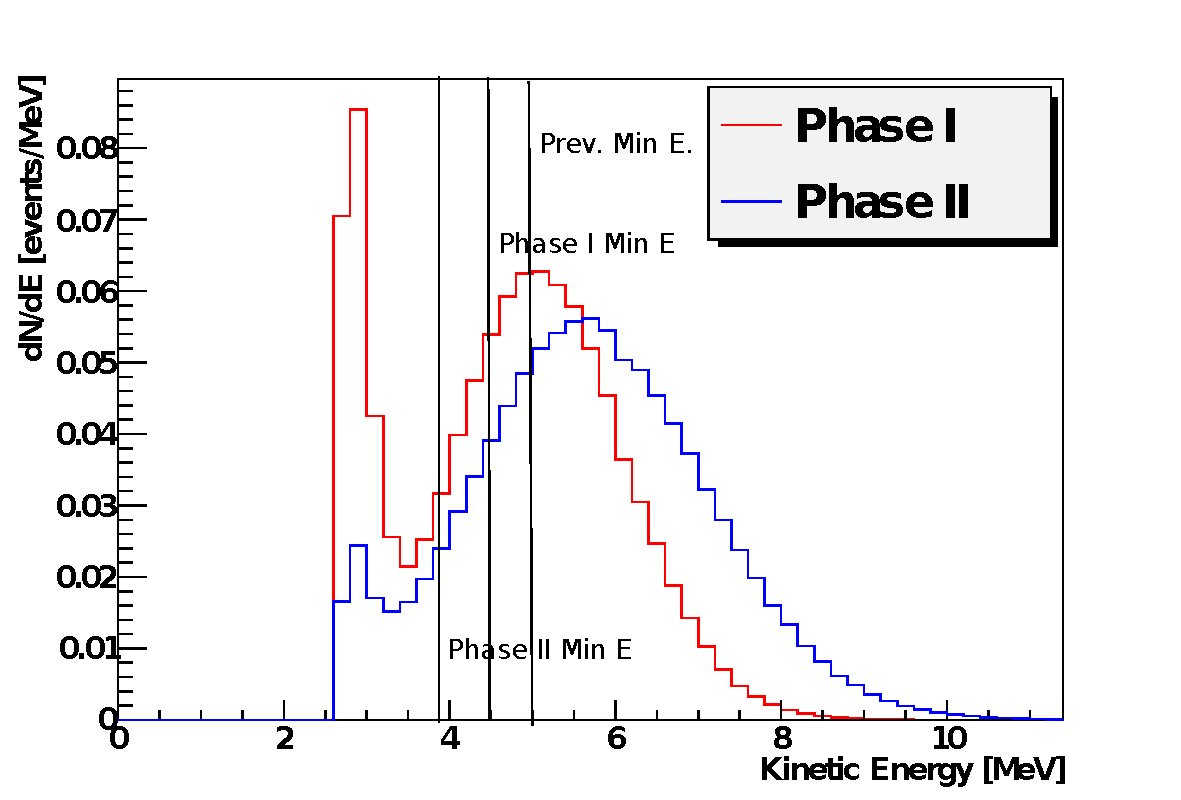
\includegraphics[width=14 cm]{nDandS.pdf} % requires the graphicx package
   \caption{The reconstructed kinetic energy of the gamma emitted after captures. The energies shown here are from simulations of neutrons in Phases I and II. The minimum energy threshold represents the analysis trigger threshold. The low energy region (near 3 MeV) in both phases is due to neutron captures on protons. The 5 MeV peak in Phase I represents the captures of neutrons on deuterons and the 6 MeV peak in Phase II represents the capture of neutrons on both chlorine and deuterons. The ratio of the capture cross-section of 35Cl to deuteron makes the deuteron capture small.}
   \label{fig:neutronEn}
\end{figure}

In the inverse beta decay reaction, the positron carries the bulk of the antineutrino kinetic energy and is approximated as the antineutrino energy minus the threshold of the interaction. In the case of inverse beta decay on deuterium the positron energy is approximated as
\begin{equation}
E_{e^+}\approx E_{\bar{\nu}}-4.03\ \mathrm{MeV}.
\end{equation}
Simulating antineutrinos from a reactor spectrum and using the Phase II detector gives the prompt and delayed energies shown in Figure \ref{fig:nuEn}.  The positron and neutron energy distributions are different and this difference can be exploited to search for these particles with different minimum analysis energy thresholds.  Specifically the positron spectrum extends lower than the neutron spectrum so using two thresholds allows for an increase in the overall acceptance of antineutrino coincidences compared to single threshold analyses while maintaing similar expected background contributions.  

\begin{figure}[htbp]
   \centering
   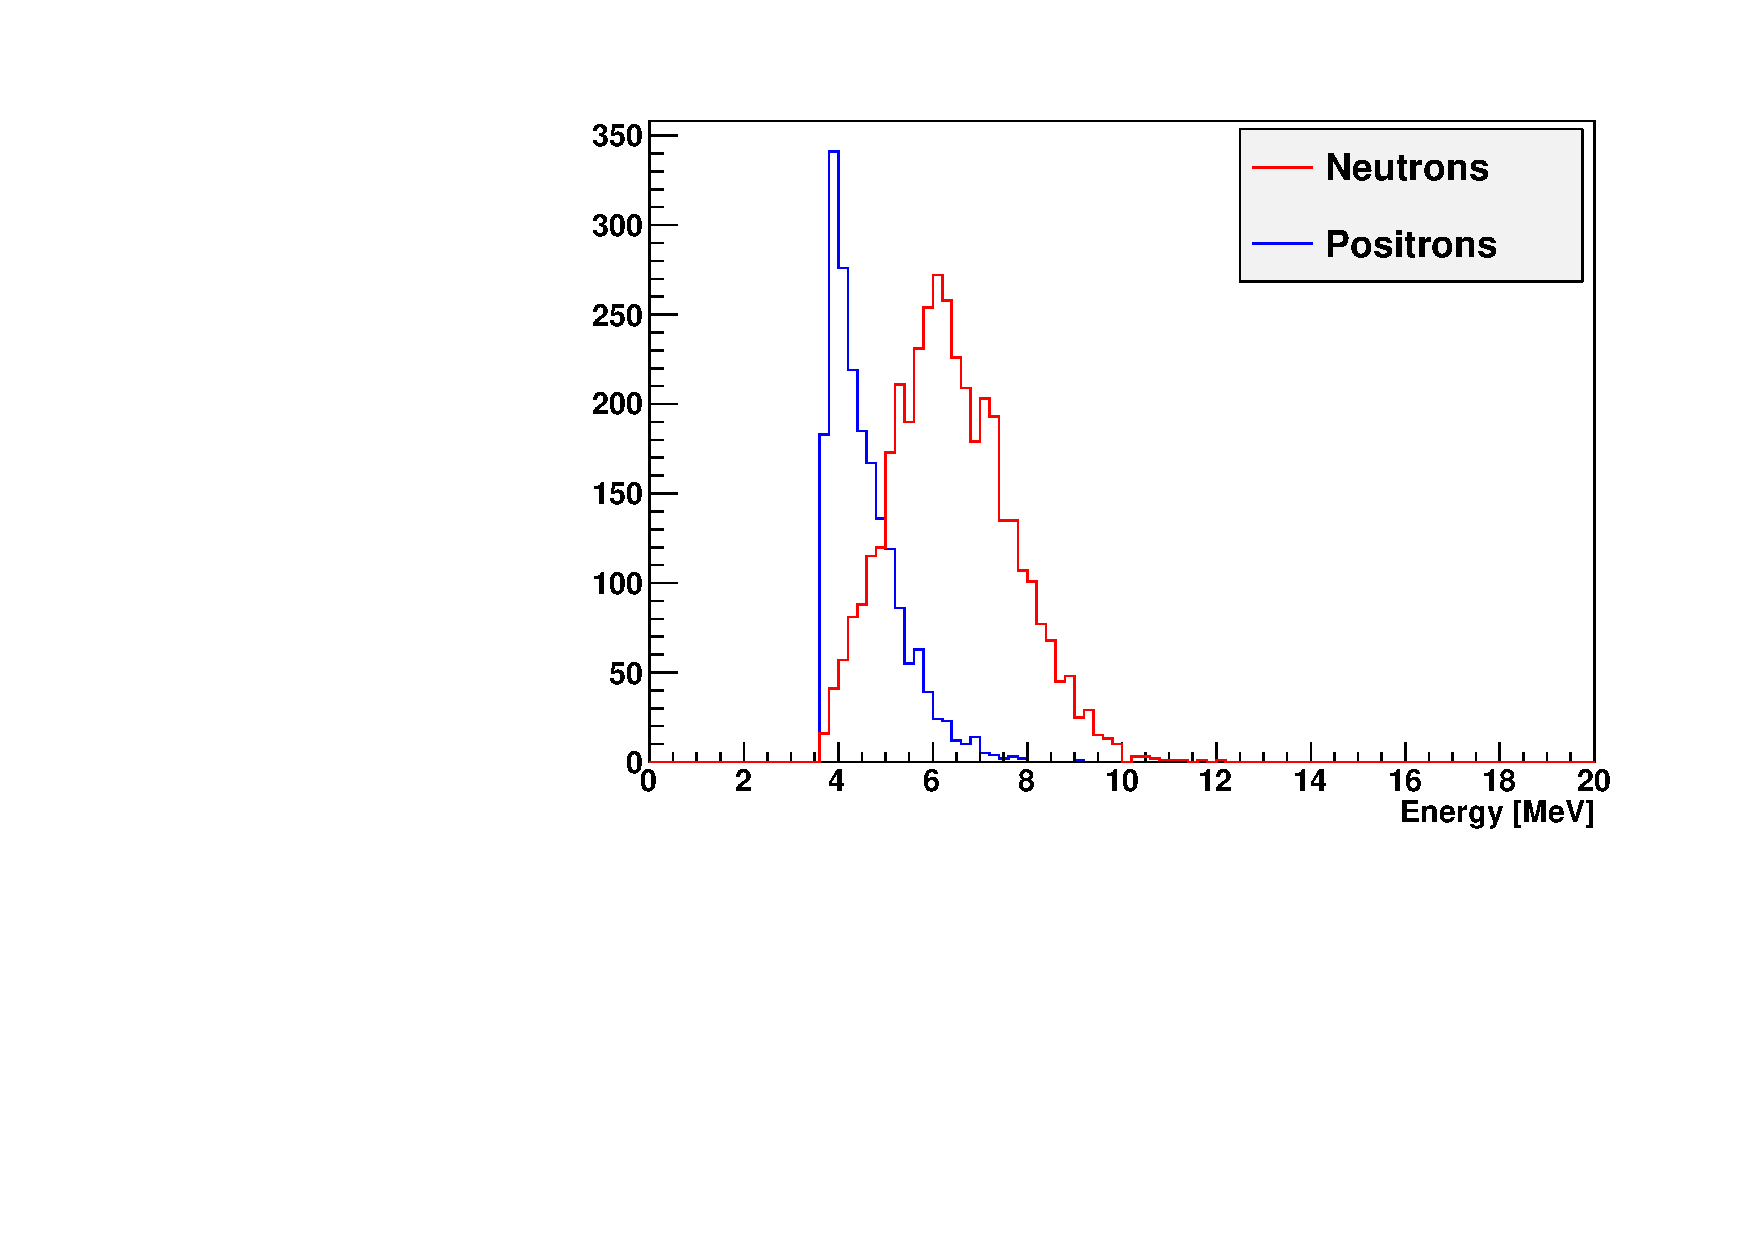
\includegraphics[width=14 cm]{energyS.pdf} % requires the graphicx package
   \caption{The visible energy distributions for events simulated using a reactor antineutrino spectrum in Phase II of SNO. The red are the delayed particles (neutrons) and the blue are the prompt particles (positrons).}
   \label{fig:nuEn}
\end{figure}

\section{Accidental Coincidences}
\label{sec:bg} 
The backgrounds in antineutrino experiments will differ depending on the detector, but one background that is consistent among all detectors is accidental coincidences.  The rate of two- and three-fold accidental coincidences  particles are given by
\begin{equation}
r_{acc}(2-fold)=r_1r_2\Delta t
\label{eq:r2}
\end{equation}
and
\begin{equation}
r_{acc}(3-fold)=r_1r_2r_3\Delta t_{12}\Delta t_{23},
\label{eq:r3}
\end{equation}
where $r_i$ is the rate of a single event and $\Delta t_{ij}$ is the size of acceptance time-window between events in a coincidence.  The rate $r_i$ and thus the total rate of accidental coincidence $r_{acc}(n-fold)$ is directly related to the minimum energy threshold used to search for particle of type $i$. If the particles in the coincidence have different energy thresholds, then the rate of single events will be different for the different particles.  In the case of reactor antineutrinos at SNO, the positron visible energy is peaked at the minimum accepted value given the software trigger threshold of 3.2 MeV, while the visible neutron energy is peaked above 6 MeV as shown in Figure \ref{fig:nuEn}. This is further illustrated in a plot of prompt and delayed energies (respectively called predecessor and primary) in Figure \ref{fig:eeS}, so applying a lower energy threshold for only the positrons will not reject many neutrons.  The two energy thresholds allows for acceptance of low energy positrons without the additional backgrounds from a low energy neutron search. 

In addition to the two energy thresholds, backgrounds can be reduced by utilized the time- and spatial-correlation of antineutrino events.  Figure \ref{fig:drdt} shows the capture time and length between prompt and delayed particles in an antineutrino coincidence. Since accidental coincidences are not spatially correlated, the two events will have a flat distribution in space and time applying a distance cut corresponding to the neutron capture length in the medium will further reduce the accidental background.  

\begin{figure}[htbp]
   \centering
   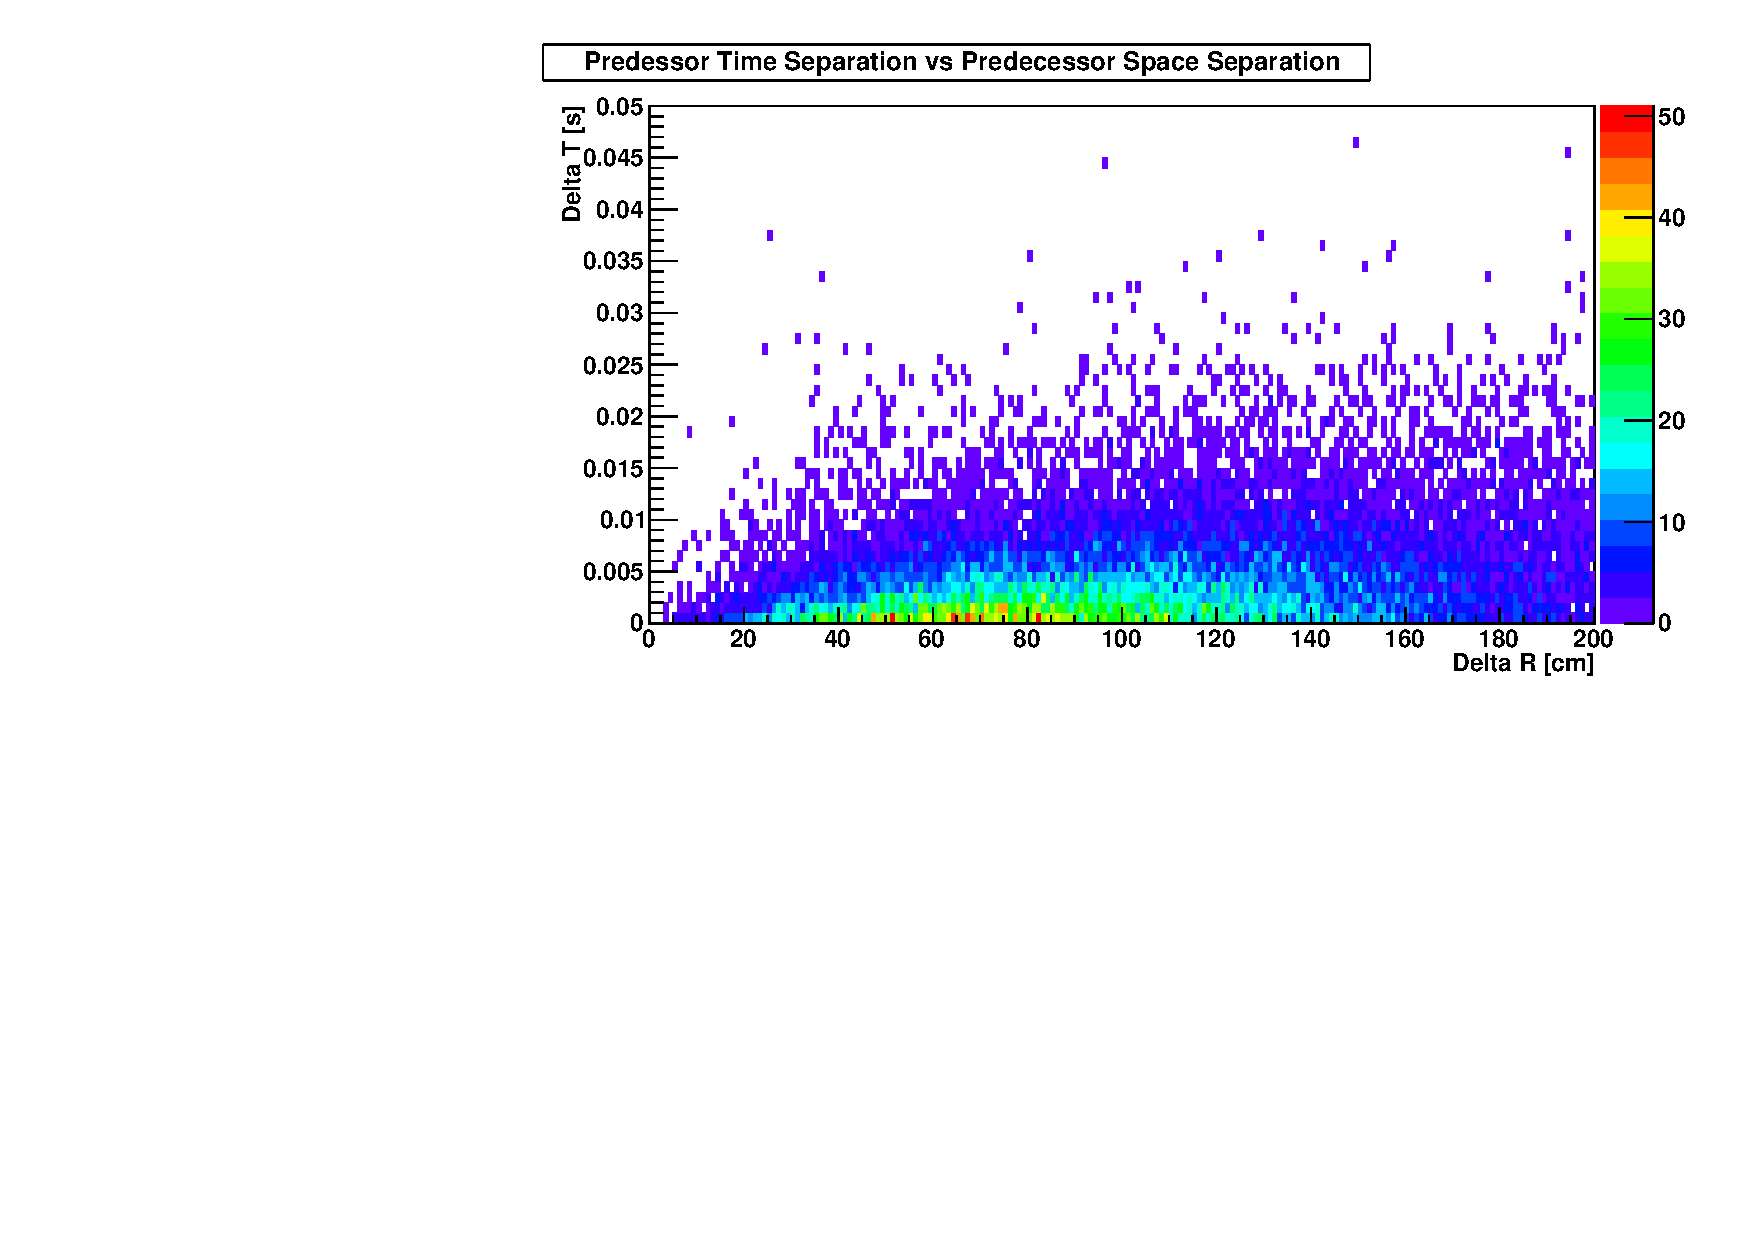
\includegraphics[width=14 cm]{drdtSMC.pdf} % requires the graphicx package
   \caption{A plot showing $\Delta r$, the reconstructed distance between prompt and delayed particles, and $\Delta t$, the time between prompt particle detection and delayed particle detection, for events generated using a reactor antineutrino spectrum in Phase II of SNO.}
   \label{fig:drdt}
\end{figure}

\begin{figure}[ht]
 \centering
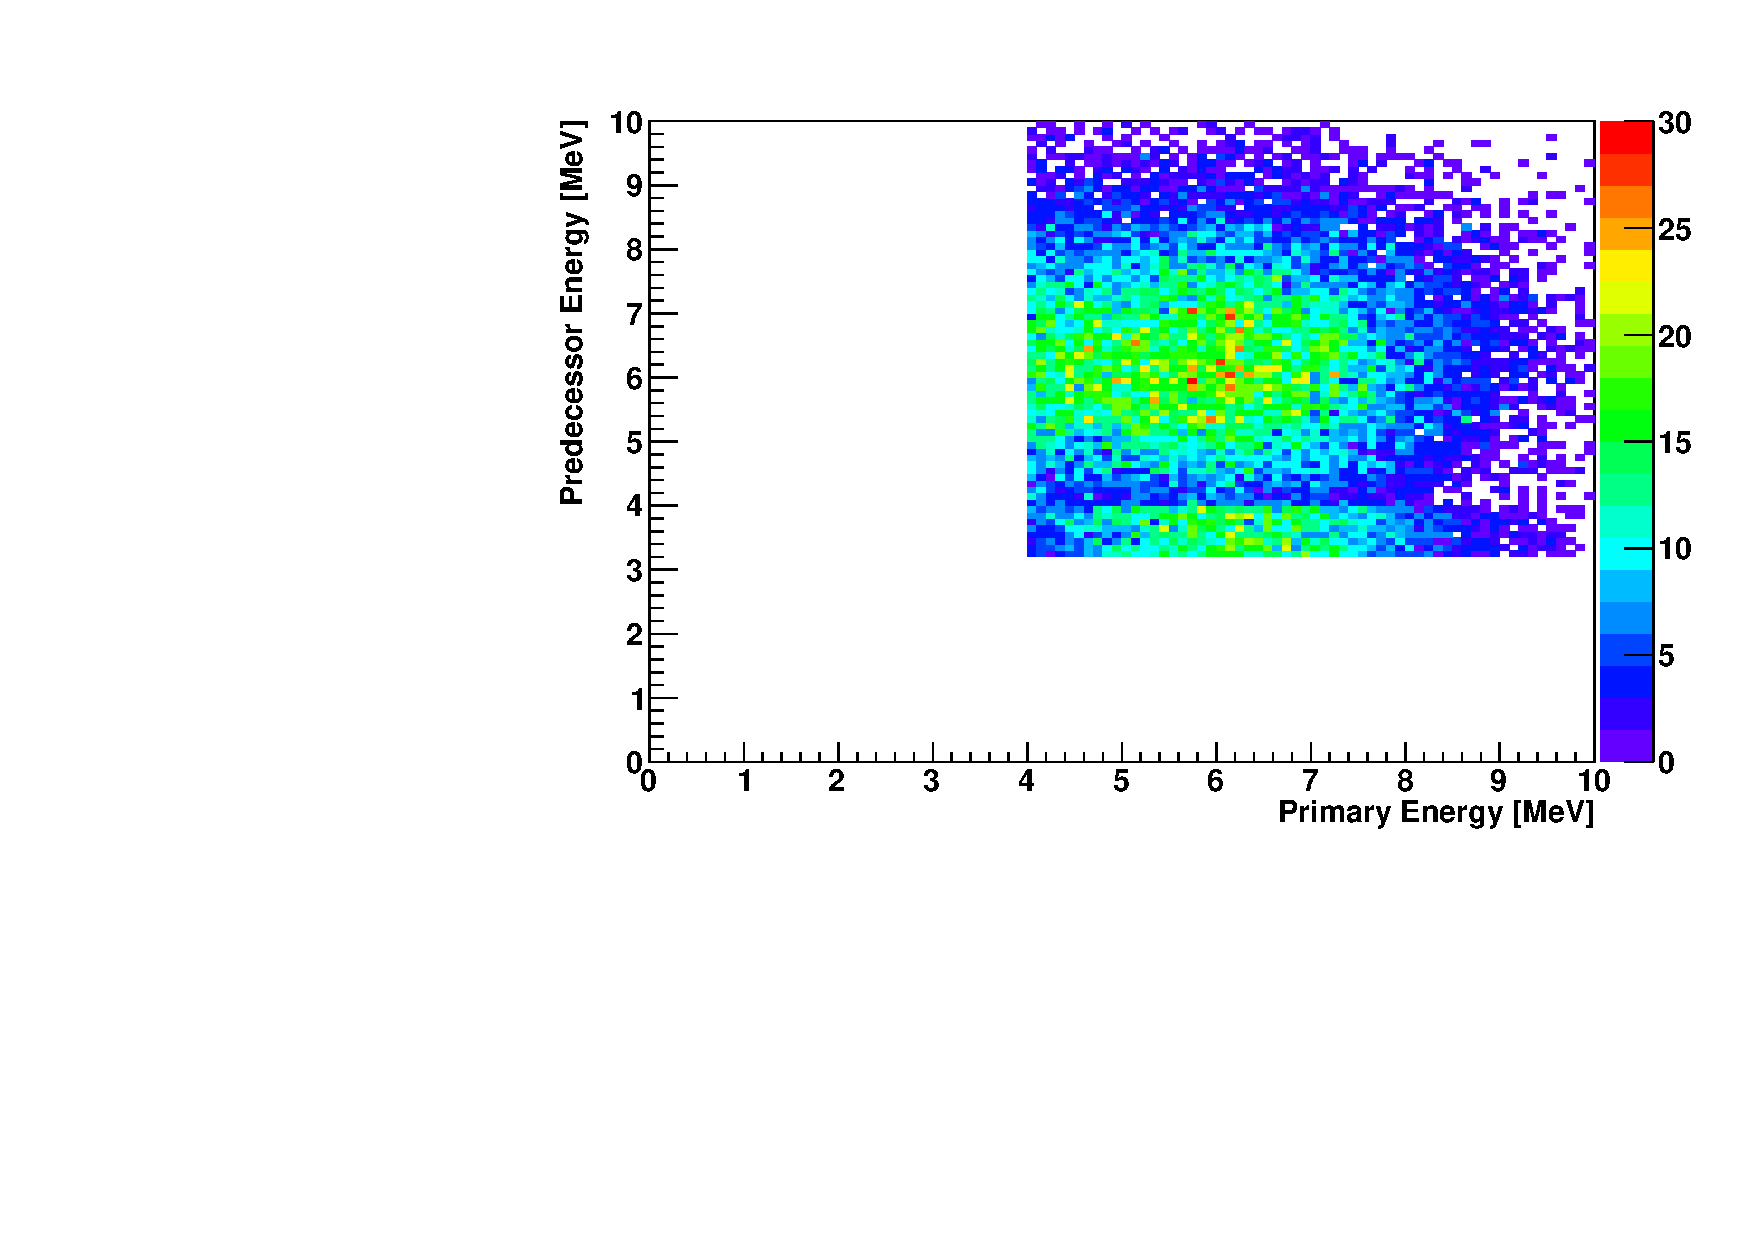
\includegraphics[width=14 cm]{eVesalt.pdf}

\caption{Energy of primary vs. predecessor energy for coincidence events in the Phase II analysis.  The region peaked at 6 MeV in both primary and predecessor likely represents two neutrons, and the region peaked at 4 MeV in predecessor energy represent a positron and neutron. The cuts represent the trigger thresholds of 2.7 MeV kinetic. } 
\label{figure:eeS}
\end{figure}

\section{Method}
\label{sec:intro} 
In water Cherenkov experiments neutrons are detected by their captures on protons, deuterons, chlorine, or gadolinium. In the case of deuterons, chlorine, and gadolinium the neutron capture cause the emission of $\gamma$s or $\gamma$ cascades, which are of energies between 6.25 and 8.6 MeV.  These visible neutron energies are peaked at higher values than positron energies from the inverse beta decay of reactor antineutrinos on either protons or deuterons. The high energy of the neutrons means that an energy threshold associated with a low single particle rate can be applied to neutron search without much neutron signal loss. 

This analysis method first searches for the neutron(s) and the looked back in time for find the lower energy positron.  In the specific case of the second phase of SNO an antineutrino can be identified by either a three-fold coincidence of the final particles in Equation \ref{eq:ivdd}, or a two-fold coincidence of either the positron and one of the neutrons or both neutrons.  The analysis code parsed through all events in data until an event above 4.5 MeV was found, this event is called the primary.  Once a primary was found, the code reset to back several events and then looked for events above 3.2 MeV that occurred within a time window (50 ms) of the primary, and continued parsing until several events after the primary. The multiplicity of the burst was then counted and events that were not two- or three-fold were rejected. The multiplicity two and three events were then subjected to a distance cut (200 cm) and coincidences were either accepted or rejected. 


\section{Results and Comparisons}
\label{sec:results}  
In a previously published SNO solar antineutrino analysis \cite{snoantinu}, the analysis was conducted using 305.9 live days of data from the first phase.  In the previously published analysis there was a single energy threshold of 5 MeV on both prompt and delayed particles.  The analysis found 2 candidate events with and expected background of $1.68^{+0.93}_{-0.45}$ events.  Using this information the SNO collaboration calculated a limit on the solar antineutrino flux of $\Phi \le 3.4\times10^4 \mathrm{\ cm^{-2}s^{-1}}$ in the 4-14.8 MeV energy range and a limit on the neutrino to antineutrino conversion probability of $4.0\times 10^{-2}$. 

Although only the Phase II analysis is discussed here, this analysis technique was applied to  all three phases of SNO, and the results are summarized in Table \ref{tab:results}.  The best limit from the look-back analysis was an order of magnitude better than the previously published limit. 

% Requires the booktabs if the memoir class is not being used
\begin{table}[htbp]
   \centering
   %\topcaption{Table captions are better up top} % requires the topcapt package
   \begin{tabular}{ccc} % Column formatting, @{} suppresses leading/trailing space

      Phase & $\Phi_{max}\mathrm{\ [cm^{-2}s^{-1}]}$ & $P(\nu\rightarrow\bar{\nu})$\\
\hline
	I & 2240 &$4.4\times10^{-4}$ \\
	II & 1710 & $3.1\times10^{-4}$\\
	III & 2210&$4.4\times10^{-4}$ \\
\hline
   \end{tabular}
   \caption{Results from a look-back analysis in each phase of SNO.}
   \label{tab:results}
\end{table}
\section{Conclusion}
\label{sec:conclusion}   

A new method for antineutrino searches in water Cherenkov detectors is described here, which utilizes two separate energy thresholds for the prompt and delayed particles. The described method is able to improve sensitivity with minimal background edition by taking advantage of the properties of true antineutrino coincidences to distinguish real events from background.  This method has been applied to data from SNO, and a solar antineutrino search was used as a test case.  Comparison to previously published single threshold analysis yielded an order of magnitude improvement to the limit of solar antineutrinos. 
%% The Appendices part is started with the command \appendix;
%% appendix sections are then done as normal sections
%% \appendix

%% \section{}
%% \label{}

%% References
%%
%% Following citation commands can be used in the body text:
%% Usage of \cite is as follows:
%%   \cite{key}          ==>>  [#]
%%   \cite[chap. 2]{key} ==>>  [#, chap. 2]
%%   \citet{key}         ==>>  Author [#]

%% References with bibTeX database:


\bibliography{bib}{}

\bibliographystyle{amsplain}
%% References without bibTeX database:

% \begin{thebibliography}{00}

%% \bibitem must have the following form:
%%   \bibitem{key}...
%%

% \bibitem{}

% \end{thebibliography}


\end{document}

%%
%% End of file `elsarticle-template-1a-num.tex'.
